\documentclass[polish,a4paper]{article}
\usepackage{amsmath}
\usepackage{amssymb, amsfonts, amsthm, amsmath, bm}
\usepackage[T1]{fontenc}
\usepackage[utf8]{inputenc}
\usepackage{babel}
\usepackage{pslatex}
\usepackage{pgfplots}
\usepackage{hhline}
\usepackage[american]{circuitikz} 
\usepackage{anysize}
\usepackage{gensymb}
\usepackage{graphicx}
\DeclareGraphicsExtensions{.jpg}
\marginsize{2.5cm}{2.5cm}{3cm}{3cm}
\bibliographystyle{IEEEtran}


%makro do indeksów w tabeli
\newcommand{\PRzFieldDsc}[1]{\sffamily\bfseries\scriptsize #1}

%makro do informacji w tabeli
\newcommand{\PRzFieldCnt}[1]{\itshape #1}

%potężne makro tworzące tabelę z informacjami o teamie
\newcommand{\PRzHeading}[8]{
%% #1 - nazwa laboratorium
%% #2 - kierunek 
%% #3 - specjalność 
%% #4 - rok studiów 
%% #5 - symbol grupy lab.
%% #6 - temat 
%% #7 - numer lab.
%% #8 - skład grupy ćwiczeniowej

\begin{center}
\begin{tabular}{ p{0.32\textwidth} p{0.15\textwidth} p{0.15\textwidth} p{0.12\textwidth} p{0.12\textwidth} }

  &   &   &   &   \\
\hline
\multicolumn{5}{|c|}{}\\[-1ex]
\multicolumn{5}{|c|}{{\LARGE #1}}\\
\multicolumn{5}{|c|}{}\\[-1ex]

\hline
\multicolumn{1}{|l|}{\PRzFieldDsc{Kierunek}}	& \multicolumn{1}{|l|}{\PRzFieldDsc{Specjalność}}	& \multicolumn{1}{|l|}{\PRzFieldDsc{Rok studiów}}	& \multicolumn{2}{|l|}{\PRzFieldDsc{Symbol grupy lab.}} \\
\multicolumn{1}{|c|}{\PRzFieldCnt{#2}}		& \multicolumn{1}{|c|}{\PRzFieldCnt{#3}}		& \multicolumn{1}{|c|}{\PRzFieldCnt{#4}}		& \multicolumn{2}{|c|}{\PRzFieldCnt{#5}} \\

\hline
\multicolumn{4}{|l|}{\PRzFieldDsc{Temat Laboratorium}}		& \multicolumn{1}{|l|}{\PRzFieldDsc{Numer lab.}} \\
\multicolumn{4}{|c|}{\PRzFieldCnt{#6}}				& \multicolumn{1}{|c|}{\PRzFieldCnt{#7}} \\

\hline
\multicolumn{5}{|l|}{\PRzFieldDsc{Skład grupy ćwiczeniowej oraz numery indeksów}}\\
\multicolumn{5}{|c|}{\PRzFieldCnt{#8}}\\

\hline
\multicolumn{3}{|l|}{\PRzFieldDsc{Uwagi}}	& \multicolumn{2}{|l|}{\PRzFieldDsc{Ocena}} \\
\multicolumn{3}{|c|}{\PRzFieldCnt{\ }}		& \multicolumn{2}{|c|}{\PRzFieldCnt{\ }} \\

\hline
\end{tabular}
\end{center}
}
%koniec potężnego makro do tabeli

\begin{document}

%stworzenie tabeli - miejsce na zmienianie danych w tabeli
%indeksy do uzupełnienia
\PRzHeading{Laboratorium Podstaw Elektroniki}{Informatyka}{--}{I}{I1}{Układy wzmacniaczy operacyjnych}{6}{Ewa Fengler(132219), Sebastian Maciejewski(132275), Jan Techner(132332)}{}

%ZADANIA

\section*{Cel}
Celem przeprowadzanych doświadczeń jest poznanie funkcji wzmacniaczy operacyjnych w układach elektronicznych.

\section{Zadanie 1.3}

\subsection*{6.}
amplitudy
\subsection*{7.}
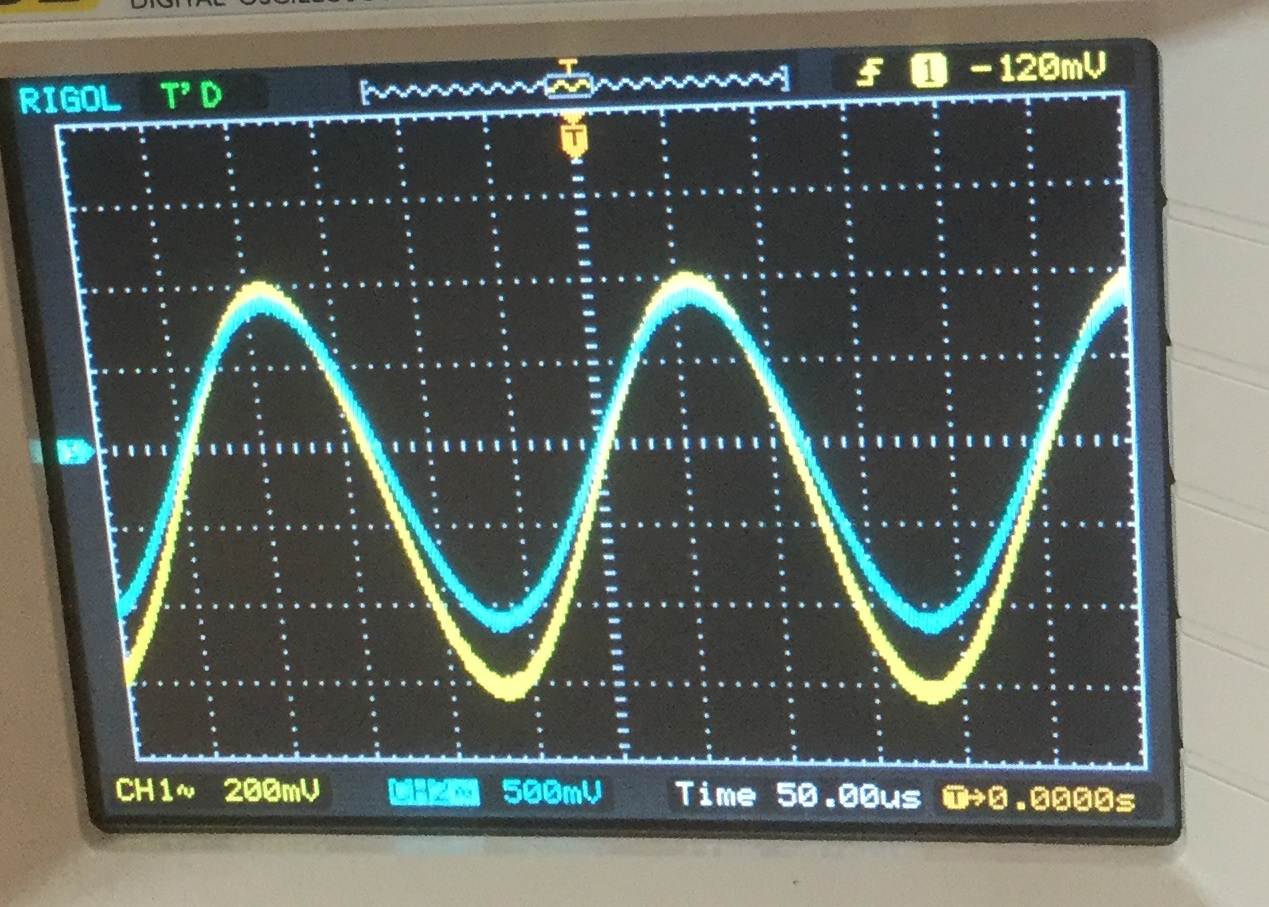
\includegraphics[scale=0.5]{amplituda}
\subsection*{8.}
Wzmocnienie: 2[V/V], w skali decybelowej: 20 log10(2) -> 6 dB
\subsection*{9.}
porównaj wzmocnienia
\subsection*{10.}
W układzie wtórnika $Z_f$ wynosi $0\Omega$, a $Z_{in}$ wynosi $\infty$ . Po podstawieniu do wzoru otrzymujemy wartość wzmocnienia równą 1. Wtórnik napięciowy stosuje się w celu separacji wejścia od wyjścia, bowiem nie obciąża on układu wejściowego (generującego napięcie wejściowe), ponieważ impedancja wejściowa wzmacniacza operacyjnego teoretycznie jest nieskończona. Równocześnie, ponieważ teoretyczna impedancja wyjściowa wzmacniacza operacyjnego wynosi 0, w związku z czym może być (teoretycznie) dowolnie obciążona.

\section{Zadanie 1.4}

\subsection*{1.}

\subsection*{4.}

\begin{center}
\begin{tabular}{|c|c|c|c||c|c|c|c|c|}
\hline
\textbf{$Z_{in}$} & \textbf{nr przełącznika} & \textbf{$Z_f$} & \textbf{nr przełącznika} & \textbf{$k_u$ teoretyczne } & \textbf{$u_we$} & \textbf{$u_wy$} & \textbf{$k_u$ [V/V]} & \textbf{$k_u$ [dB] } \\ 
\hhline{|=|=|=|=#=|=|=|=|=|}
$k_u$ teoretyczne & $u_we$ & $u_wy$ & $k_u$ & ...\\ %w dB z tego wzoru gdzieś wyżej
$1k\Omega$ & 1 & $2k\Omega$ & 1 & -2 [V/V] & 0,5 V & 1V & -2 & ...\\
\hline
$1k\Omega$ & 1 & $1k\Omega$ & 2 & -1 [V/V] & 0,5 V & 0,5V & -1 & ...\\
\hline
$1k\Omega$ & 1 & $5k1\Omega$ & 3 & -5,1[V/V] & 100mV & 0,5V & -5 & ...\\
\hline
$2k\Omega$ & 2 & $1k\Omega$ & 2 & -0,5[V/V] & 1V & 0,5V & -0,5 & ...\\
\hline

\end{tabular}
\end{center}


\subsection*{5.}
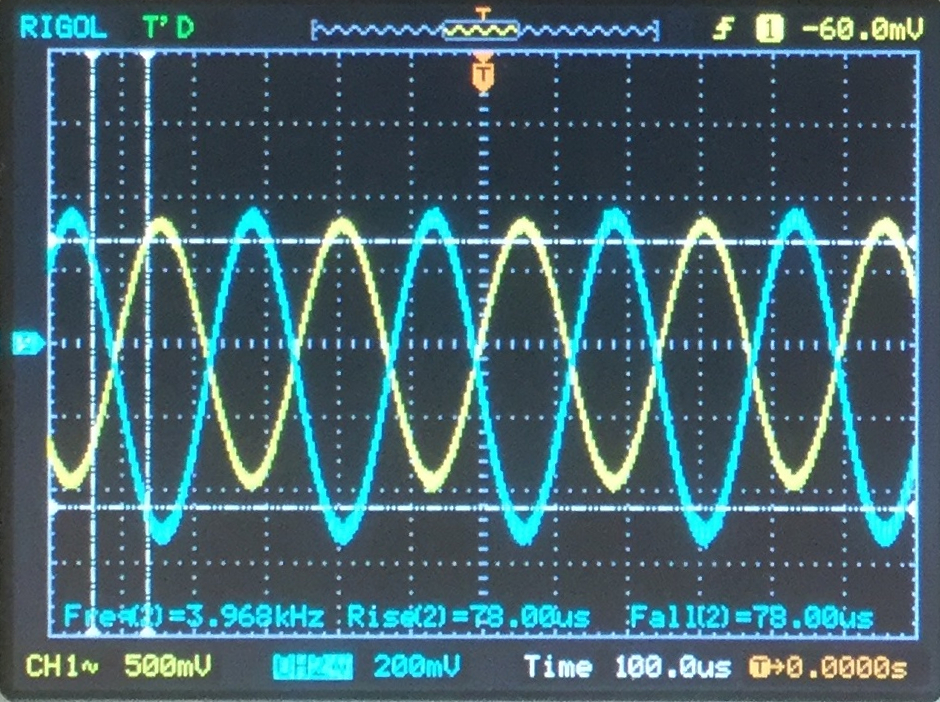
\includegraphics[scale=0.5]{czestotliwosc}
\subsection*{6.}
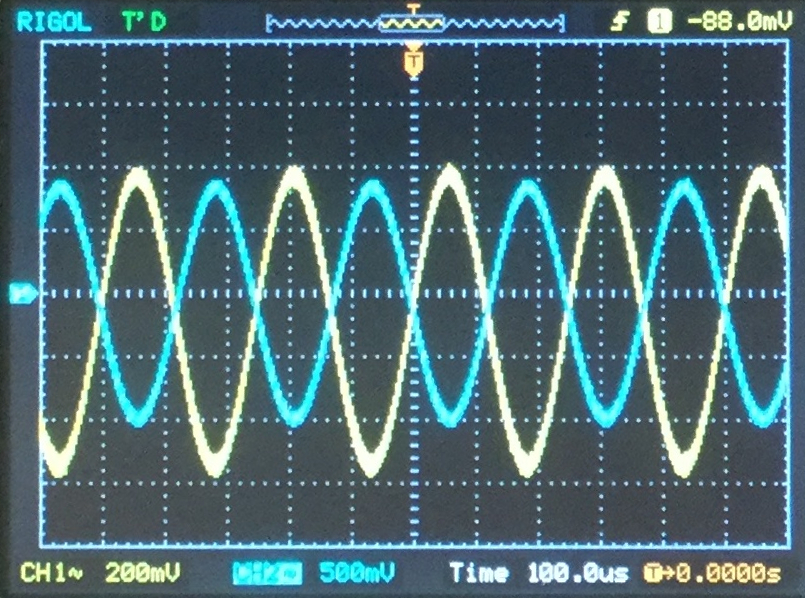
\includegraphics[scale=0.5]{k_odwracajaca}
\subsection*{7.}
Różnice zostały stwierdzone dla wzmocnienia 5,1[V/V] i są spowodowane błędem pomiaru. Szacowany błąd odczytu wartości napięcia amplitudy na oscyloskopie wynosi około 5% (jedna działka do wartości międzyszczytowej - 1/20), powoduje to, że wartość teoretyczna mieści się w przedziale błędu pomiaru (4,75[V/V] - 5,25[V/V]). 
\subsection*{8.}
Przesunięcie fazowe między przebiegami wynosi $180\degree$ i jest spowodowane podaniem sygnału na wejście odwracające wzmacniacza operacyjnego.


\section{Zadanie 1.5}

\subsection*{1.}
schemat?
\subsection*{4.}
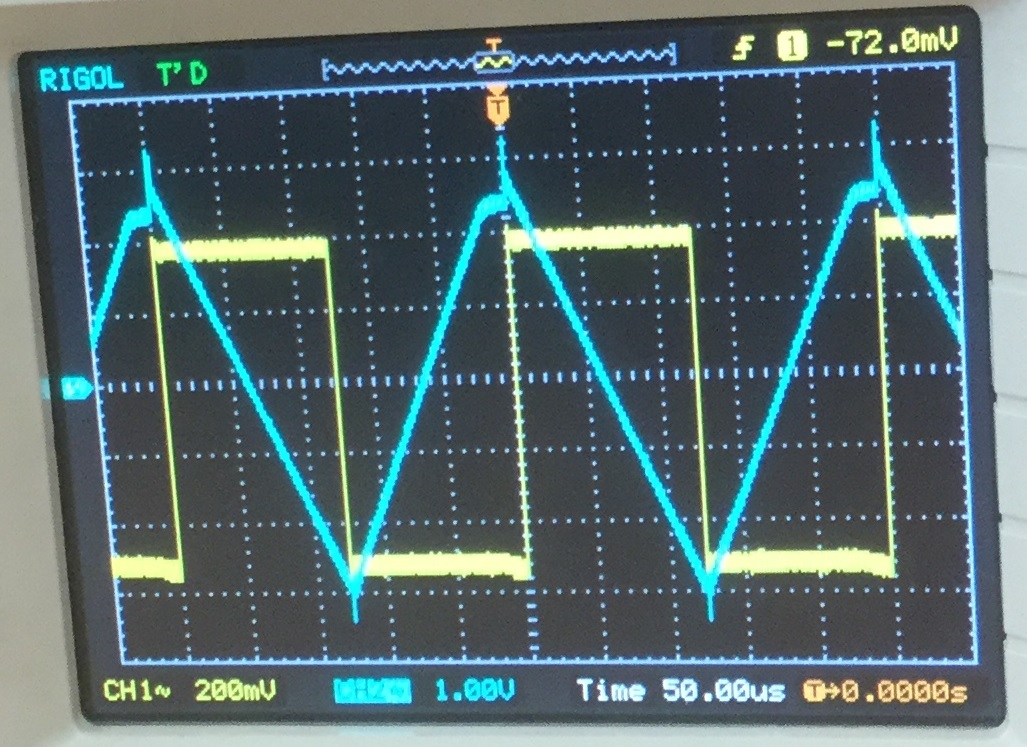
\includegraphics[scale=0.5]{przebieg_trojkatny}
\subsection*{5.}
zdjęcie i obliczenie nachylenia
1. Wiersz tabeli: 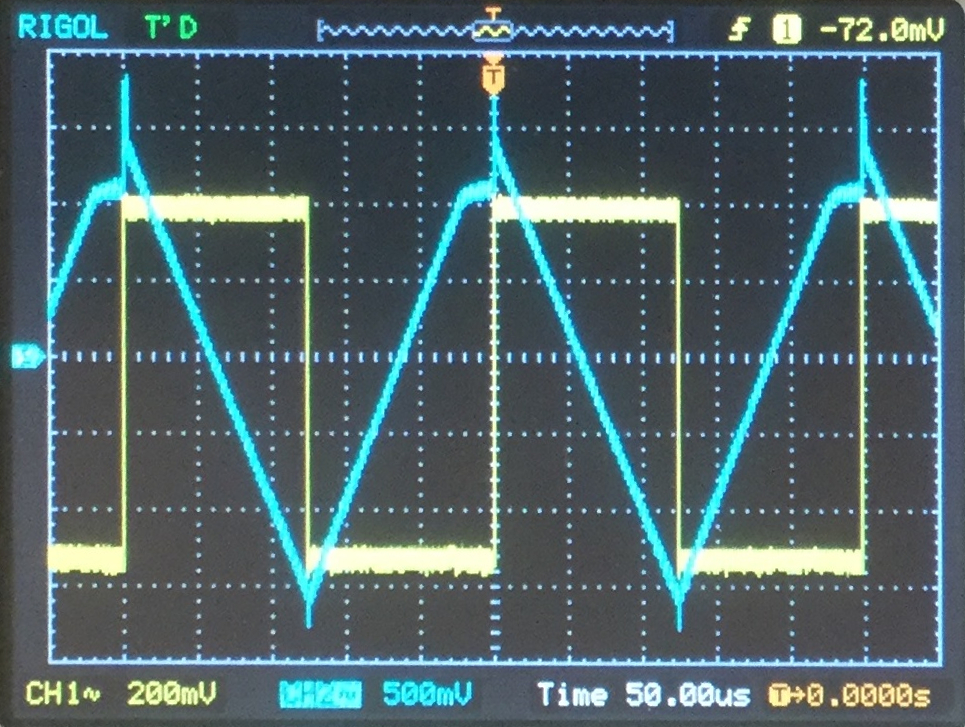
\includegraphics[scale=0.5]{r1c4}\\
2. Wiersz tabeli: 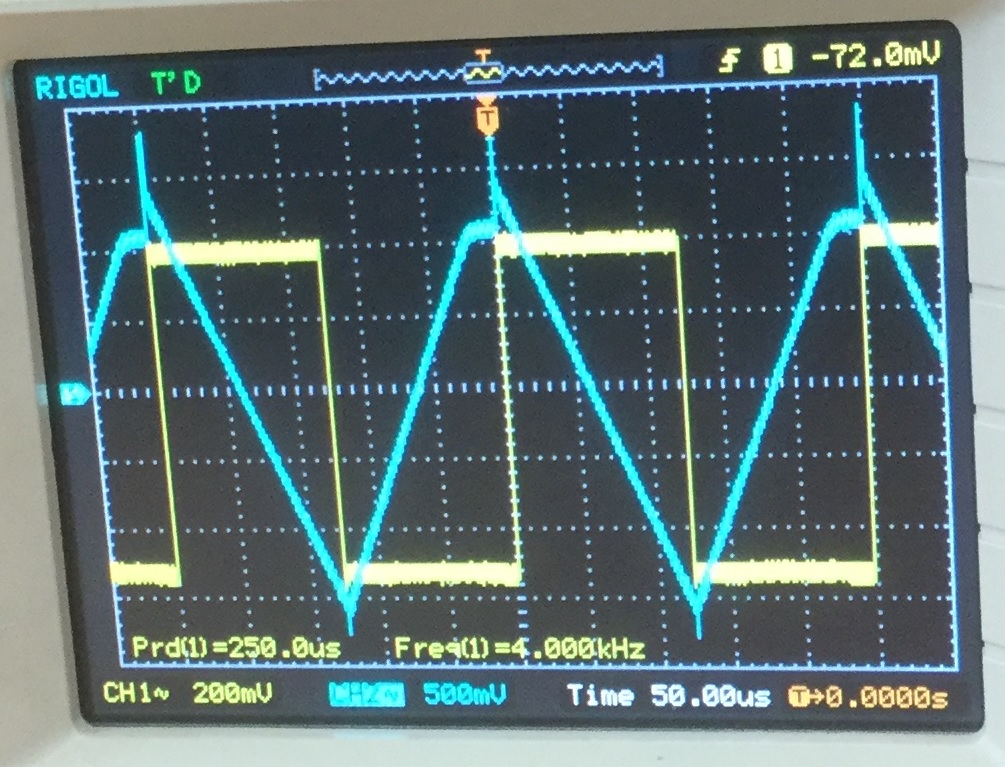
\includegraphics[scale=0.5]{r2c4}
\subsection*{6.}
tabelka?
\subsection*{7.}
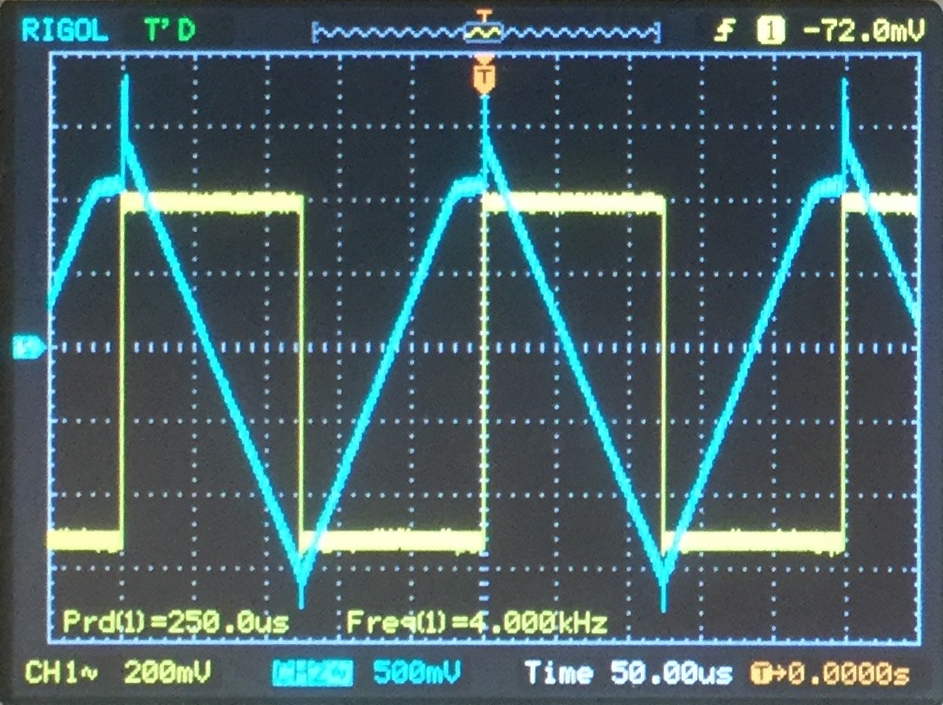
\includegraphics[scale=0.5]{czestotliwosc2}
\subsection*{8.}
Przykładowy oscylogram pary przebiegów:
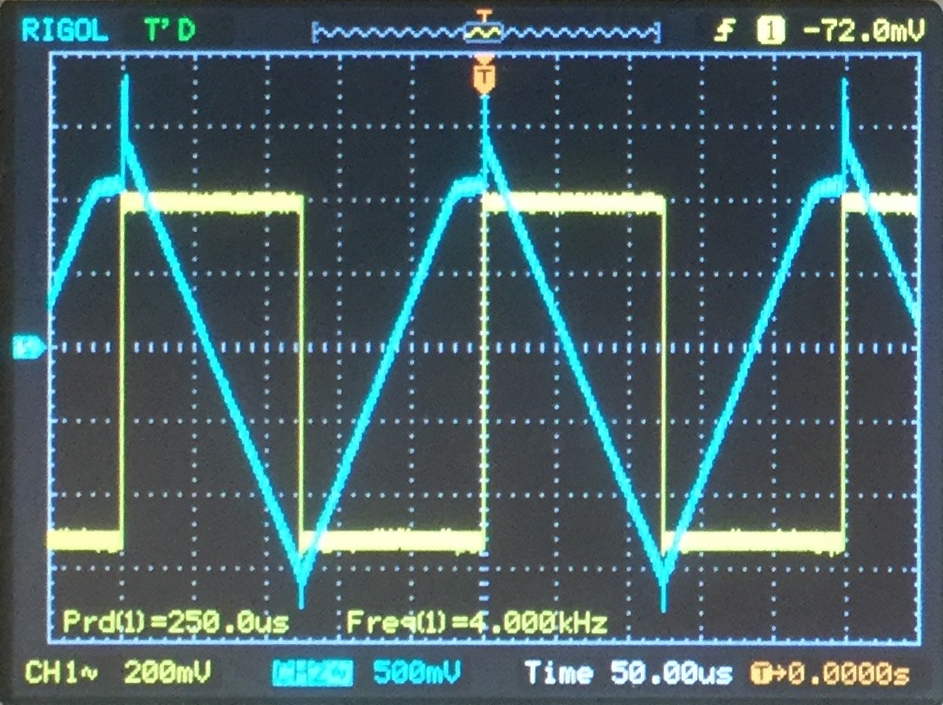
\includegraphics[scale=0.5]{czestotliwosc2}

\section{Zadanie 1.6}

\subsection*{1.}
schemat?
\subsection*{4.}
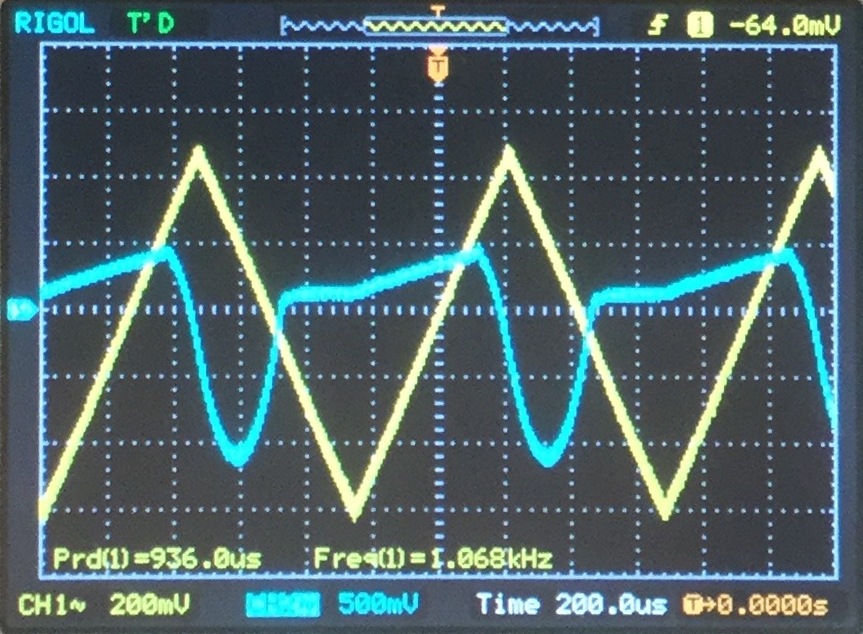
\includegraphics[scale=0.5]{czestotliwosc3}
\subsection*{5.}
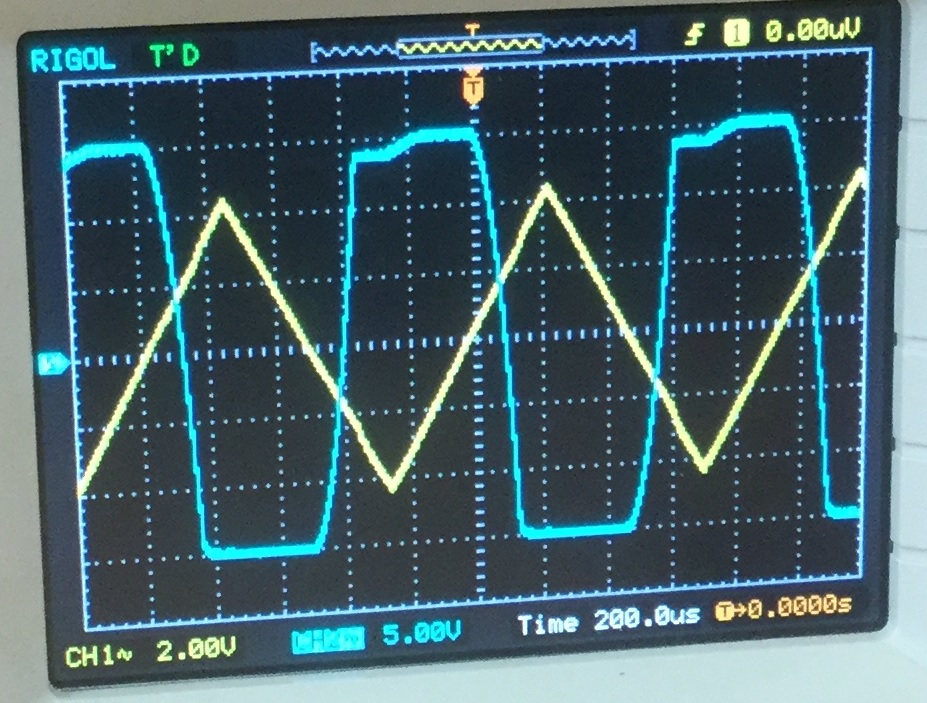
\includegraphics[scale=0.5]{lepiej}
\subsection*{6.}
Lepiej: 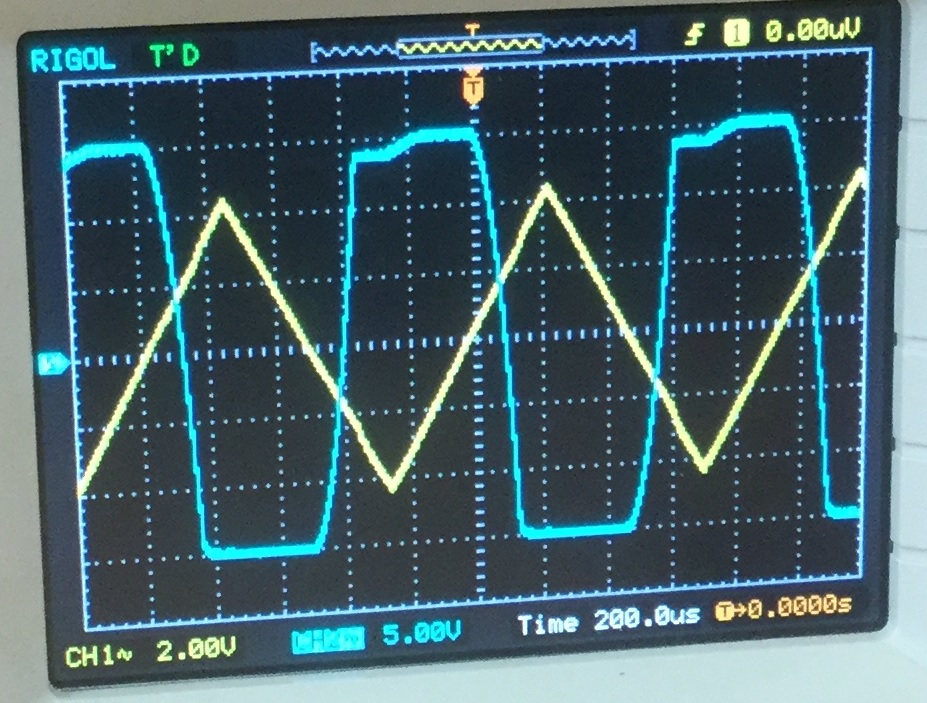
\includegraphics[scale=0.5]{lepiej}\\
Gorzej: 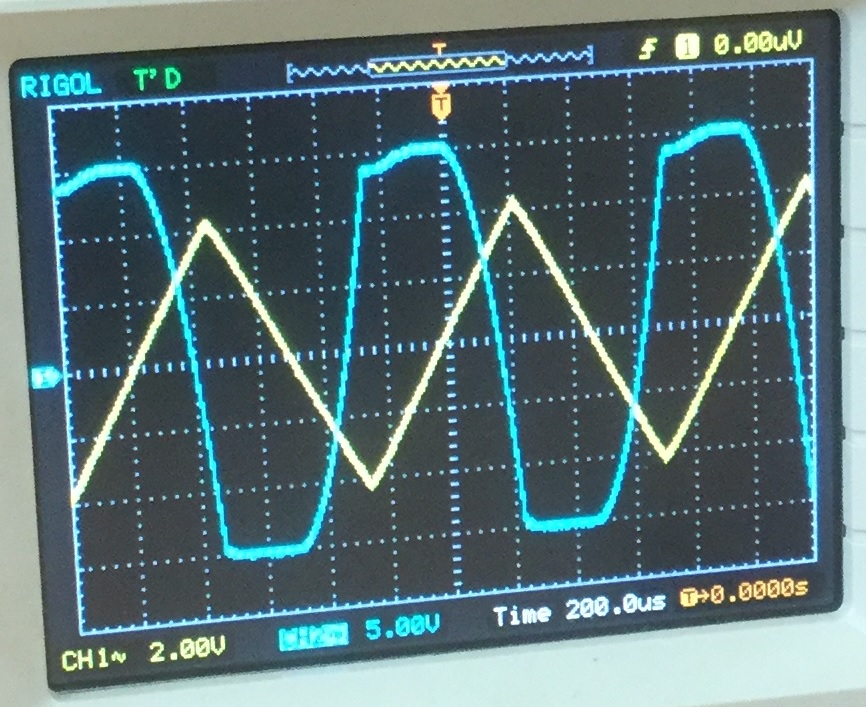
\includegraphics[scale=0.5]{gorzej}
\subsection*{7.}
Na przebiegu wyjściowym układu różniczkującego obserwujemy 2 rodzaje zniekształceń. Pierwsze zniekształcenie polega na ograniczonej prędkości narastania i opadania zbocza przebiegu wyjściowego. Wynika to z ograniczeń wzmacniacza operacyjnego, którego jedną z cech katalogowych jest maksymalna prędkość narastania napięcia wyjściowego (niezależne od charakterystyk częstotliwościowych). Drugie zniekształcenie wynika z pracy wzmacniacza w nasyceniu, napięcia maksymalne są równe napięciu zasilania wzmacniacza operacyjnego. Zasadniczo przebieg prostokątny otrzymano przede wszystkim ze względu na nasycenie, a w mniejszym stopniu ze względu na różniczkowanie sygnału przez układ badany.
Teoretycznie powinniśmy uzyskać zniekształcenia polegające na podwzbudzaniu wzmacniacza operacyjnego (zafalowania części płaskich) wynikające ze zbliżania się układu ze sprzeżeniem zwrotnym do stanu niestabilnego (kryterium Nyquista).


\bibliography{IEEEabrv,refs}

\begin{thebibliography}{9}

\bibitem{rlc}
  W trakcie przeprowadzania doświadczeń i pisania sprawozdania zespół korzystał głównie z materiałów ze strony http://mariusznaumowicz.ddns.net/materialy.html oraz z wiedzy własnej.\\


\end{thebibliography}

\end{document}7